\chapter{तरल की शुद्धगतिकी}\label{ch:b2:fluid-kinematics}

किसी पुल पर खड़े होकर नदी देखिए। एक पत्ता बहता हुआ आता है, खंभों के बीच
तेज़ हो जाता है, नीचे के कुंड में धीमा पड़ता है, किसी भँवर में एक चक्कर
काटता है और आगे बढ़ जाता है। आप नदी का वर्णन उस पत्ते के पीछे चलकर कर
सकते हैं --- हर क्षण उसकी स्थिति और वेग लिखकर --- या फिर स्थिर खड़े रहकर,
नदी के हर बिंदु पर यह लिखकर कि वहाँ पानी कितनी तेज़ी से गुज़रता है। दूसरा
वर्णन तरल-भौतिकी वाले का है: एक \emph{वेग क्षेत्र}।
यह अध्याय दोनों वर्णन खड़े करता है, क्षेत्र से किसी कण का
त्वरण निकालना सिखाता है, द्रव्यमान-संरक्षण को स्थानिक नियम के रूप में
लिखता है, और प्रवाहों को इस आधार पर बाँटता है कि वे घूमते हैं या नहीं ---
अर्थात् वह सारी शब्दावली, जो ऑयलर और नेवियर के समीकरणों को चाहिए होगी।

\begin{omfigure}
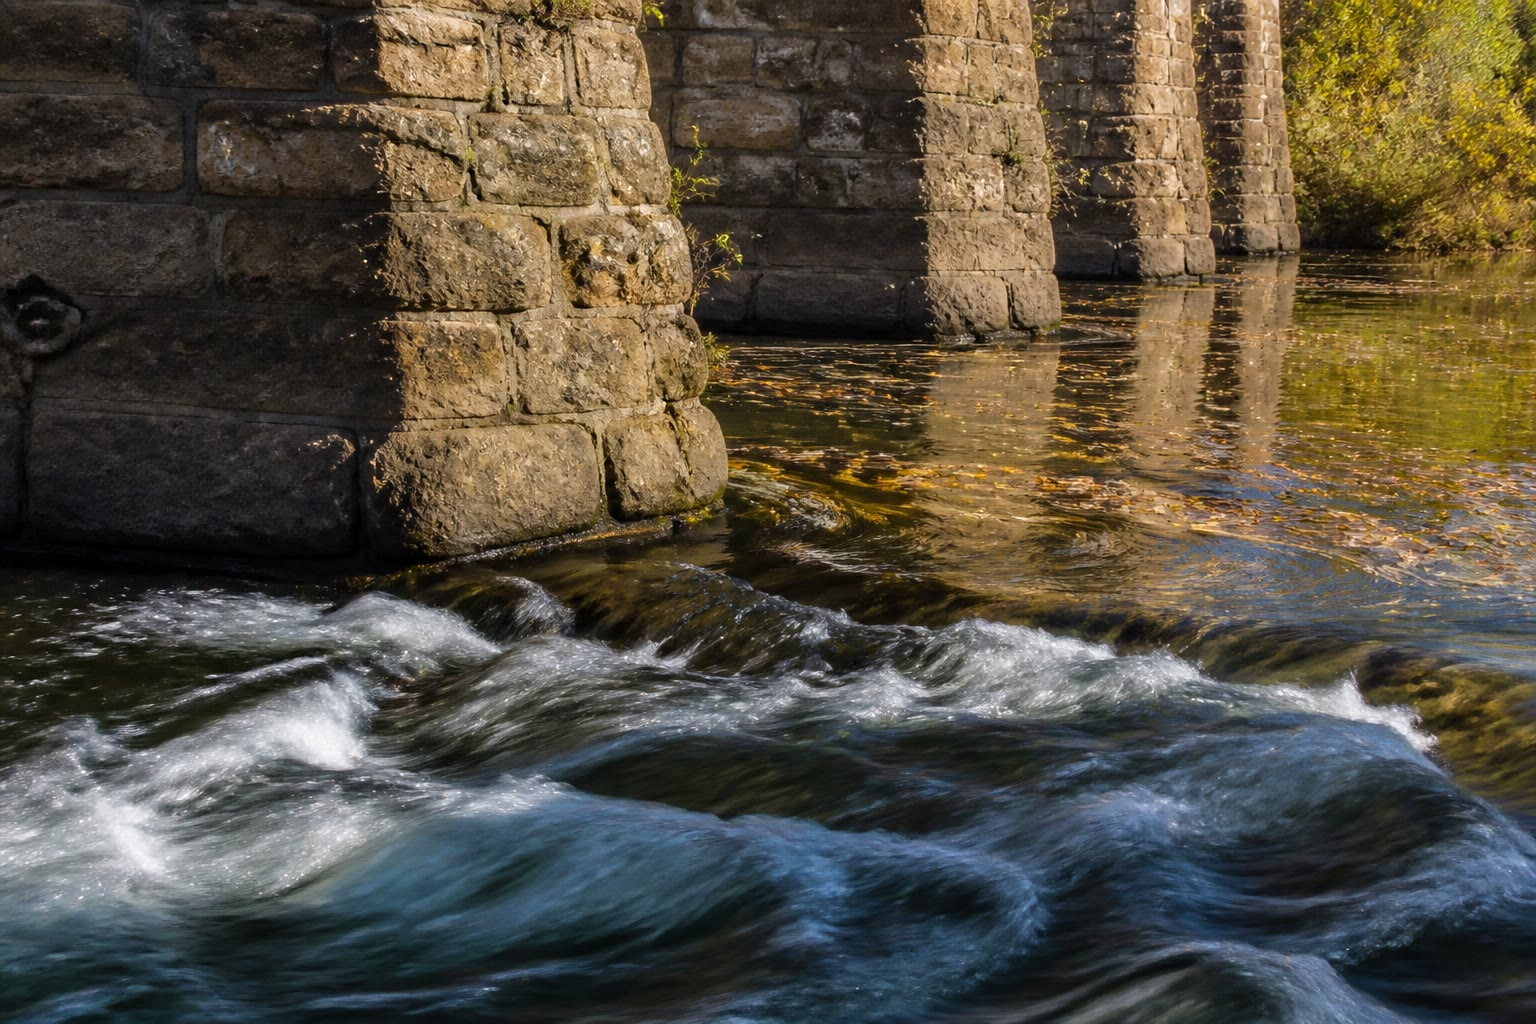
\includegraphics[width=0.58\linewidth]{images/book4/ai/b4-02-river-bridge-eddies.jpg}

{\small पुल के पास नदी: खंभों के बीच तेज़ और चिकना पानी, उनकी ओट में भँवर --- अर्थात् एक वेग क्षेत्र, जिसे स्थिर बिंदुओं पर पढ़ना है, न कि कोई एक प्रक्षेप-पथ, जिसके पीछे चलना है।}
\end{omfigure}


\section{सांतत्य-वर्णन}

\begin{definition}[तरल कण; सांतत्य परिकल्पना]\label{def:b2:fluid-kinematics:particle}
\index{तरल कण}\index{सांतत्य परिकल्पना}\index{मध्यदर्शी पैमाना}
\emph{तरल कण} तरल का इतना छोटा आयतन है कि प्रवाह के पैमाने पर उसे बिंदु
माना जा सके, फिर भी इतना बड़ा कि उसमें अणुओं की विशाल
संख्या रहे, और इसलिए उसका घनत्व $\rho$, दाब $P$,
ताप $T$ तथा माध्य वेग $\vect v$ सुपरिभाषित औसत हों
(\emph{मध्यदर्शी} पैमाना, प्रायः एक माइक्रोमीटर)। \emph{सांतत्य
परिकल्पना} यह मानती है कि ऐसा कोई पैमाना है: अणुओं का माध्य मुक्त पथ $\ell$
प्रवाह के पैमाने $L$ से बहुत छोटा होना चाहिए,
$\ell/L \ll 1$। वायुमंडलीय दाब पर हवा में $\ell \approx \qty{70}{nm}$; किसी
द्रव में $\ell$ अणु के आकार का होता है। तब तरल का वर्णन हर बिंदु पर
परिभाषित \emph{क्षेत्रों} $\rho(M, t)$, $P(M, t)$, $\vect v(M, t)$ से होता है।
\end{definition}

\begin{definition}[लाग्रांजीय और ऑयलरीय वर्णन]\label{def:b2:fluid-kinematics:euler}
\index{लाग्रांजीय वर्णन}\index{ऑयलरीय वर्णन}\index{धारा-रेखा}\index{पथ-रेखा}\index{स्थायी प्रवाह}
\emph{लाग्रांजीय} वर्णन हर \omterm{def:b2:fluid-kinematics:particle}{तरल कण} के पीछे चलता है: समय और कण की आरंभिक
स्थिति के फलन के रूप में उसकी स्थिति $\vect r(t)$ और वेग $\dd\vect r/\dd t$।
\emph{ऑयलरीय} वर्णन हर स्थिर
बिंदु $M$ और समय $t$ पर उस कण का वेग $\vect v(M, t)$ देता है, जो
उस क्षण $M$ से होकर गुज़र रहा है। \emph{पथ-रेखा}
किसी कण का प्रक्षेप-पथ है; समय $t$ पर \emph{धारा-रेखा} वह
वक्र है जो हर बिंदु पर $\vect v(M, t)$ की स्पर्शरेखा हो; और
\emph{धारा-नलिका} किसी बंद वक्र से होकर जाती धारा-रेखाओं से बना पृष्ठ है।
प्रवाह \emph{स्थायी} तब कहलाता है जब ऑयलरीय क्षेत्र समय पर
निर्भर न करें, $\partial\vect v/\partial t = \vect 0$; तब धारा-रेखाएँ और पथ-रेखाएँ
संपाती और अचल होती हैं।
\end{definition}

\begin{example}[एक ही प्रवाह के दो वर्णन]\label{ex:b2:fluid-kinematics:hose}
$S$ काट वाली बगीचे की नली में $Q$ प्रवाह दर पर पानी हर जगह $v = Q/S$
से चलता है: ऑयलरीय क्षेत्र एकसमान है और हर कण की
लाग्रांजीय गति भी एकसमान। पतली होती टोंटी में ऑयलरीय क्षेत्र
अब भी स्थायी है, पर अक्ष के अनुदिश $v$ बढ़ता जाता है: हर कण गुज़रते
समय \emph{त्वरित} होता है, यद्यपि किसी स्थिर
बिंदु पर समय के साथ कुछ नहीं बदलता। \omterm{def:b2:fluid-kinematics:euler}{ऑयलरीय वर्णन} को सबसे पहले यही
व्यक्त करना सीखना है।
\end{example}

\begin{omfigure}
\begin{tikzpicture}[font=\small, x=1cm, y=1cm, >=Stealth]
  \begin{scope}
    % streamlines of a converging channel
    \foreach \y in {-1.2,-0.6,0,0.6} {
      \draw[omDef, thick, postaction={decorate, decoration={markings, mark=at position 0.55 with {\arrow{>}}}}]
        (-2.8,\y) .. controls (-0.8,\y) and (0.2,{0.45*\y}) .. (2.8,{0.45*\y});
    }
    \draw[omDef, thick, postaction={decorate, decoration={markings, mark=at position 0.55 with {\arrow{>}}}}]
        (-2.8,1.2) .. controls (-0.8,1.2) and (0.2,0.54) .. (2.8,0.54)
        coordinate[pos=0.15] (P1) coordinate[pos=0.6] (P2) coordinate[pos=0.9] (P3);
    \draw[thick] (-2.8,1.6) .. controls (-0.8,1.6) and (0.2,0.75) .. (2.8,0.75);
    \draw[thick] (-2.8,-1.6) .. controls (-0.8,-1.6) and (0.2,-0.75) .. (2.8,-0.75);
    \fill[omThm] (P1) circle (2pt) node[above, font=\footnotesize, yshift=1pt] {$t_1$};
    \fill[omThm] (P2) circle (2pt) node[above, font=\footnotesize, yshift=1pt] {$t_2$};
    \fill[omThm] (P3) circle (2pt) node[above, font=\footnotesize, yshift=1pt] {$t_3$};
    \node[font=\footnotesize, align=center] at (0,-2.15) {स्थायी प्रवाह: धारा-रेखाएँ $=$ पथ-रेखाएँ,\\नलिका जहाँ सँकरी होती है वहाँ कण तेज़ होता है};
  \end{scope}
  \begin{scope}[xshift=7.4cm]
    \draw[thick,->] (-2.8,-1.2) -- (2.8,-1.2) node[right, font=\footnotesize] {$x$};
    \draw[thick,->] (-2.8,-1.2) -- (-2.8,1.6);
    % velocity vectors at fixed points (Eulerian)
    \foreach \x in {-2.2,-1.2,-0.2,0.8,1.8} \foreach \y in {-0.6,0.2,1.0} {
      \draw[omDef, ->] (\x,\y) -- ({\x+0.5+0.12*\x},{\y+0.15*\y});
    }
    \node[omDef, font=\footnotesize] at (0,1.75) {ऑयलरीय: स्थिर बिंदुओं पर $\vect v(M,t)$};
    \draw[omThm, thick, ->] (-2.5,-0.9) .. controls (-1,-0.3) and (0.5,0.9) .. (2.4,1.3);
    \node[omThm, font=\footnotesize] at (2.2,0.7) {पथ-रेखा};
    \node[font=\footnotesize, align=center] at (0,-1.95) {लाग्रांजीय: एक कण के पीछे चलिए};
  \end{scope}
\end{tikzpicture}

{\small बाएँ: स्थायी अभिसारी प्रवाह --- \omterm{def:b2:fluid-kinematics:euler}{धारा-रेखाएँ} अचल हैं,
कोई चिह्नित कण उनमें से एक पर चलता है और नलिका के सँकरे होते ही
त्वरित होता है। दाएँ: \omterm{def:b2:fluid-kinematics:euler}{ऑयलरीय वर्णन} स्थिर बिंदुओं पर वेग सदिश
लिखता है; \omterm{def:b2:fluid-kinematics:euler}{लाग्रांजीय वर्णन} किसी एक कण के पीछे उसकी
\omterm{def:b2:fluid-kinematics:euler}{पथ-रेखा} पर चलता है।}
\end{omfigure}

\section{द्रव्य अवकलज}

\begin{theorem}[द्रव्य (कण) अवकलज]\label{thm:b2:fluid-kinematics:material}
\index{द्रव्य अवकलज}\index{संवहनी त्वरण}
किसी राशि $G(M, t)$ (अदिश या सदिश) के परिवर्तन की दर, उस
\emph{\omterm{def:b2:fluid-kinematics:particle}{तरल कण} के लिए} जो $M$ से होकर समय $t$ पर गुज़र रहा है,
\[
\frac{\mathrm DG}{\mathrm Dt} = \frac{\partial G}{\partial t} + (\vect v\cdot
\operatorname{\vect{grad}})\,G ,
\qquad\text{तथा विशेषतः}\qquad
\vect a = \frac{\mathrm D\vect v}{\mathrm Dt} = \frac{\partial\vect v}{\partial t} +
(\vect v\cdot\operatorname{\vect{grad}})\,\vect v ,
\]
होती है, जहाँ $(\vect v\cdot\operatorname{\vect{grad}}) = v_x\partial_x + v_y\partial_y +
v_z\partial_z$ है। पहला पद परिवर्तन की \emph{स्थानिक} दर है (किसी
स्थिर बिंदु पर), दूसरा \emph{संवहनी} दर (क्योंकि कण वहाँ चला जाता है
जहाँ $G$ भिन्न है)। वेग के लिए, $(\vect v\cdot
\operatorname{\vect{grad}})\vect v = \operatorname{\vect{grad}}(v^2/2) +
(\operatorname{\vect{curl}}\vect v)\wedge\vect v$।
\end{theorem}

\begin{proof}
$\dd t$ में कण $M$ से $M + \vect v\,\dd t$ तक जाता है, अतः प्रथम कोटि तक
$\dd G =
G(M + \vect v\dd t, t + \dd t) - G(M, t) = \partial_tG\,\dd t + \dd t\,(v_x\partial_x
+ v_y\partial_y + v_z\partial_z)G$ (चार चरों वाले फलन का
शृंखला-नियम)। सदिश-सर्वसमिका $x$ घटक पर जाँची जाती
है: $[\operatorname{\vect{grad}}(v^2/2)]_x = v_x\partial_xv_x + v_y\partial_x
v_y + v_z\partial_xv_z$ और $[(\operatorname{\vect{curl}}\vect v)\wedge\vect v]_x =
v_y(\partial_yv_x - \partial_xv_y) + v_z(\partial_zv_x - \partial_xv_z)$ (जहाँ
$\operatorname{\vect{curl}}\vect v$ के घटक नीचे
\cref{def:b2:fluid-kinematics:vorticity} में दिए हैं); इनका योग $v_x\partial_xv_x +
v_y\partial_yv_x + v_z\partial_zv_x$ है।
\end{proof}

\begin{example}[स्थायी टोंटी में त्वरण]\label{ex:b2:fluid-kinematics:nozzle}
किसी टोंटी के अनुदिश एक-विमीय \omterm{def:b2:fluid-kinematics:euler}{स्थायी प्रवाह} $v(x) = v_0(1 + x/L)$:
स्थानिक पद लुप्त हो जाता है, और $a = v\,\dd v/\dd x = v_0^2(1 + x/L)/L$। कोई
कण $v_0 = \qty{2}{m/s}$ पर घुसता है और $2v_0$ पर निकलता है; $L
= \qty{5}{cm}$ की इस दूरी में वह $a = 80$ से \qty{160}{m/s^2} तक अनुभव करता है: अर्थात् आठ से सोलह गुना $g$, और वह भी ऐसे
प्रवाह में जहाँ कुछ भी समय पर निर्भर नहीं।
\end{example}

\begin{example}[स्थानिक बनाम संवहनी]\label{ex:b2:fluid-kinematics:weather}
किसी मौसम-केंद्र पर रात में ताप गिरता है ($\partial T/
\partial t < 0$: स्थानिक), और हवा जिस वायु-पिंड को उत्तर की ओर ले जाती है
उसका ताप भी गिरता है ($\vect v\cdot\operatorname{\vect{grad}}T < 0$: संवहनी, या
\emph{अभिवहनी})। हवा के साथ बहते गुब्बारे पर लगा तापमापी
दोनों का योग, $\mathrm DT/\mathrm Dt$, लिखता है; मौसम-केंद्र केवल
पहला पद लिखता है।
\end{example}

\section{द्रव्यमान का संरक्षण}

\begin{definition}[द्रव्यमान प्रवाह दर और आयतन प्रवाह दर]\label{def:b2:fluid-kinematics:flowrate}
\index{द्रव्यमान प्रवाह दर}\index{आयतन प्रवाह दर}\index{द्रव्यमान अभिवाह}
किसी दिष्ट पृष्ठ $S$ से होकर \emph{द्रव्यमान प्रवाह दर} वह द्रव्यमान है
जो उसे प्रति एकांक समय में पार करता है, $D_m = \sum\rho\,\vect v\cdot\vect n\,\dd S$ ---
अर्थात् \emph{द्रव्यमान धारा घनत्व} $\vect j = \rho\vect v$ का अभिवाह (मात्रक
\unit{kg.m^{-2}.s^{-1}}); और \emph{आयतन प्रवाह दर} $D_V = \sum\vect v
\cdot\vect n\,\dd S$ (\unit{m^3/s}) है। $S$ क्षेत्रफल की किसी समतल काट के
अभिलंब एकसमान वेग के लिए, $D_m = \rho vS$ और $D_V = vS$।
\end{definition}

\begin{proof}
$\dd t$ में अवयव $\dd S$ को पार करता तरल वही है जो
$\dd S$ आधार और $\vect v\,\dd t$ जनक वाले तिरछे बेलन में समाया है, जिसका
आयतन $\vect v\cdot\vect n\,\dd S\,\dd t$ और द्रव्यमान उसका $\rho$ गुना है।
\end{proof}

\begin{theorem}[द्रव्यमान का स्थानिक संरक्षण]\label{thm:b2:fluid-kinematics:continuity}
\index{सांतत्य समीकरण}\index{अपसरण}
किसी तरल के हर बिंदु पर,
\[
\frac{\partial\rho}{\partial t} + \operatorname{div}(\rho\vect v) = 0 ,
\qquad\text{जहाँ}\qquad
\operatorname{div}\vect A = \frac{\partial A_x}{\partial x} + \frac{\partial A_y}{\partial y} +
\frac{\partial A_z}{\partial z}
\]
किसी सदिश क्षेत्र का \emph{अपसरण} है: अर्थात् किसी छोटे आयतन के पृष्ठ से
$\vect A$ का बाहर जाता कुल अभिवाह, प्रति एकांक आयतन।
समतुल्य रूप से $\mathrm D\rho/\mathrm Dt + \rho\operatorname{div}\vect v = 0$।
\end{theorem}

\begin{proof}
स्थिर संदूक $[x, x + \dd x]\times[y, y + \dd y]\times[z, z + \dd z]$ लीजिए।
उसका द्रव्यमान $\rho\,\dd x\dd y\dd z$ $\partial_t\rho\,\dd x\dd y
\dd z$ की दर से बदलता है। द्रव्यमान $x$ वाले फलक से $j_x(x)\dd y\dd z$ दर से घुसता है
और $x + \dd x$ वाले फलक से $j_x(x + \dd x)\dd y\dd z$ दर से निकलता है:
अतः कुल निर्गम $\partial_xj_x\,\dd x\dd y\dd z$, और इसी तरह $y$ तथा $z$ के लिए।
द्रव्यमान का संरक्षण --- कोई द्रव्यमान बनता नहीं --- $\partial_t\rho = -
(\partial_xj_x + \partial_yj_y + \partial_zj_z)$ देता है। दूसरा रूप
$\operatorname{div}(\rho\vect v) = \vect v\cdot\operatorname{\vect{grad}}\rho +
\rho\operatorname{div}\vect v$ से निकलता है।
\end{proof}

\begin{remark}[अपसरण से पहली भेंट]\label{rem:b2:fluid-kinematics:divergence}
यह व्युत्पत्ति दिखाती है कि $\operatorname{div}$ क्या मापता है: किसी छोटे
संदूक से निकलता अभिवाह, प्रति एकांक आयतन। किसी परिमित आयतन $V$ को
भरने वाले संदूकों पर योग लेने पर भीतरी फलक जोड़े-जोड़े में कट जाते हैं और
केवल बाहरी पृष्ठ बचता है: $\iint_{\partial V}\vect A\cdot\vect n\,\dd S = \iiint_V
\operatorname{div}\vect A\,\dd\tau$ --- अर्थात् अपसरण (ऑस्ट्रोग्रैडस्की)
प्रमेय, जिसे हम \cref{ch:b2:maxwell-equations} में ठीक से रखेंगे
और पूरे विद्युत्चुंबकत्व में काम में लेंगे; उसकी उपपत्ति वर्ष 3 के
गणित-खंड में है। किसी स्थिर आयतन पर समाकलित करने पर स्थानिक नियम यह पढ़ा जाता है:
$\dd m_V/\dd t = -D_m^{\text{निर्गम}}$, अर्थात् भीतर का द्रव्यमान उतना ही
बदलता है जितना सीमा को पार करता है।
\end{remark}

\begin{omfigure}
\begin{tikzpicture}[font=\small, x=1cm, y=1cm, >=Stealth]
  \begin{scope}
    \draw[thick, fill=omDef!10] (0,0) rectangle (2.2,1.6);
    \draw[thick] (0,1.6) -- (0.6,2.1) -- (2.8,2.1) -- (2.2,1.6);
    \draw[thick] (2.2,0) -- (2.8,0.5) -- (2.8,2.1);
    \draw[omThm, very thick, ->] (-1.2,0.8) -- (-0.1,0.8) node[pos=0.3, above, font=\footnotesize] {$j_x(x)$};
    \draw[omThm, very thick, ->] (2.3,0.8) -- (3.6,0.8) node[pos=0.75, above, font=\footnotesize] {$j_x(x+\dd x)$};
    \node[font=\footnotesize] at (1.1,-0.35) {$\dd x$};
    \node[font=\footnotesize] at (-0.35,0.3) {$\dd y$};
    \node[font=\footnotesize] at (2.75,-0.05) {$\dd z$};
    \node[font=\footnotesize, align=left] at (1.3,-1.1) {$\partial_t\rho\,\dd\tau = -(\partial_x j_x + \partial_y j_y + \partial_z j_z)\,\dd\tau$};
  \end{scope}
  \begin{scope}[xshift=8.2cm]
    \draw[thick] (-2.4,1.1) .. controls (-1,1.1) and (0,0.5) .. (2.4,0.5);
    \draw[thick] (-2.4,-1.1) .. controls (-1,-1.1) and (0,-0.5) .. (2.4,-0.5);
    \draw[omDef, thick] (-2.4,0) ellipse (0.25 and 1.1);
    \draw[omDef, thick] (2.4,0) ellipse (0.12 and 0.5);
    \draw[omThm, very thick, ->] (-2.4,0) -- (-1.4,0) node[above, font=\footnotesize] {$v_1$};
    \draw[omThm, very thick, ->] (2.4,0) -- (3.6,0) node[above, font=\footnotesize] {$v_2$};
    \node[omDef, font=\footnotesize] at (-2.4,1.45) {$S_1$};
    \node[omDef, font=\footnotesize] at (2.4,0.85) {$S_2$};
    \node[font=\footnotesize] at (0,-1.6) {स्थायी: $\rho_1v_1S_1 = \rho_2v_2S_2$};
  \end{scope}
\end{tikzpicture}

{\small बाएँ: किसी स्थिर संदूक का द्रव्यमान-संतुलन --- उसके छह फलकों से
बाहर जाता कुल अभिवाह, प्रति एकांक आयतन, $\rho\vect v$ का अपसरण है।
दाएँ: \omterm{def:b2:fluid-kinematics:euler}{स्थायी प्रवाह} में किसी धारा-नलिका की हर काट से \omterm{def:b2:fluid-kinematics:flowrate}{द्रव्यमान प्रवाह
दर} एक ही रहती है।}
\end{omfigure}

\begin{corollary}[असंपीड्य प्रवाह; धारा-नलिकाएँ]\label{cor:b2:fluid-kinematics:incompressible}
\index{असंपीड्य प्रवाह}
प्रवाह \emph{असंपीड्य} तब कहलाता है जब हर कण का घनत्व अचर रहे,
$\mathrm D\rho/\mathrm Dt = 0$, जो इसके तुल्य है:
\[
\operatorname{div}\vect v = 0 .
\]
समांगी द्रव असंपीड्य रूप से बहता है; और ध्वनि की चाल से काफ़ी नीचे की
चालों पर गैस भी (देखिए \cref{ch:b2:sound-waves})। \omterm{def:b2:fluid-kinematics:euler}{स्थायी
प्रवाह} में \omterm{def:b2:fluid-kinematics:flowrate}{द्रव्यमान प्रवाह दर} $\rho vS$ धारा-नलिका की हर काट से एक ही
रहती है; और यदि प्रवाह असंपीड्य भी हो तथा $\rho$ एकसमान,
तो $vS$ अचर होता है: अर्थात् नलिका जहाँ सँकरी होती है वहाँ तरल तेज़ हो जाता है।
\end{corollary}

\begin{proof}
$\mathrm D\rho/\mathrm Dt = -\rho\operatorname{div}\vect v$। नलिका के लिए,
दो काटों के बीच के आयतन पर समाकलित संतुलन लगाइए: पार्श्व पृष्ठ से कोई
अभिवाह नहीं (वेग स्पर्शरेखीय), और स्थायी अवस्था, अतः
आगम निर्गम के बराबर है।
\end{proof}

\begin{example}[रक्त]\label{ex:b2:fluid-kinematics:blood}
महाधमनी (काट \qty{2.5}{cm^2}) \qty{5}{L/min} $= \qty{83}{cm^3/s}$ ले जाती है:
$v = \qty{33}{cm/s}$। वही प्रवाह लगभग $10^{10}$
केशिकाओं से होकर जाता है, जिनकी कुल काट लगभग \qty{2500}{cm^2} है: $v = \qty{0.3}{mm/s}$ ---
अर्थात् दीवारों से आदान-प्रदान के लिए पर्याप्त धीमा, और यही शाखान का प्रयोजन है।
\end{example}

\section{भ्रमिलता और अघूर्णी प्रवाह}

\begin{definition}[भ्रमिलता]\label{def:b2:fluid-kinematics:vorticity}
\index{भ्रमिलता}\index{कर्ल}\index{अघूर्णी प्रवाह}
किसी प्रवाह की \emph{भ्रमिलता} वह सदिश क्षेत्र है
\[
\vect\omega = \operatorname{\vect{curl}}\vect v , \qquad
\operatorname{\vect{curl}}\vect A = \Bigl(\frac{\partial A_z}{\partial y} -
\frac{\partial A_y}{\partial z},\; \frac{\partial A_x}{\partial z} - \frac{\partial A_z}
{\partial x},\; \frac{\partial A_y}{\partial x} - \frac{\partial A_x}{\partial y}\Bigr) .
\]
जहाँ $\vect\omega = \vect 0$ हो, वहाँ प्रवाह \emph{अघूर्णी} कहलाता है।
\end{definition}

\begin{proposition}[भ्रमिलता स्थानिक घूर्णन मापती है]\label{prop:b2:fluid-kinematics:rotation}
$M$ पर केंद्रित कोई छोटा तरल अवयव समग्र रूप से कोणीय वेग
$\vect\Omega = \tfrac12\vect\omega(M)$ से घूमता है। ठोस-पिंड
घूर्णन $\vect v = \vect\Omega\wedge\vect{OM}$ में \omterm{def:b2:fluid-kinematics:vorticity}{भ्रमिलता} एकसमान होती है,
$\vect\omega = 2\vect\Omega$; और समतल अपरूपण प्रवाह $\vect v = ky\,\vect e_x$
में वह $\vect\omega = -k\vect e_z$ है: अपरूपण प्रवाह में डाला गया छोटा
पंखी-चक्र घूमता है, यद्यपि \omterm{def:b2:fluid-kinematics:euler}{धारा-रेखाएँ} सीधी हैं।
\end{proposition}

\begin{proof}
$M$ के पास, $\vect v(M + \vect\epsilon) = \vect v(M) + \mathbf G\vect\epsilon$, जहाँ
$\mathbf G$ $\partial_jv_i$ का आव्यूह है; उसे सममित भाग
(शुद्ध विकृति, जो अवयव को खींचती है पर समग्र रूप से घुमाती नहीं)
और विषम-सममित भाग में बाँटिए, जिसका आव्यूह $\tfrac12(\partial_jv_i -
\partial_iv_j)$ है और वही $\vect\epsilon \mapsto \tfrac12\vect\omega\wedge\vect\epsilon$ का भी आव्यूह है
(\cref{thm:b2:rigid-body-mechanics:field})। $\vect e_z$ के परितः ठोस घूर्णन:
$\vect v = \Omega(-y, x, 0)$, $\omega_z = \partial_xv_y - \partial_yv_x = 2\Omega$।
अपरूपण: $\omega_z = -\partial_y(ky) = -k$।
\end{proof}

\begin{definition}[वेग विभव; परिचालन]\label{def:b2:fluid-kinematics:potential}
\index{वेग विभव}\index{परिचालन (वेग का)}\index{विभव प्रवाह}
\omterm{def:b2:fluid-kinematics:vorticity}{अघूर्णी प्रवाह} में वेग किसी \emph{वेग
विभव} से व्युत्पन्न होता है: $\vect v = \operatorname{\vect{grad}}\varphi$ (तब किसी पथ पर
$\vect v$ का परिचालन केवल पथ के सिरों पर निर्भर करता है, $\int_A^B\vect v
\cdot\dd\vect l = \varphi(B) - \varphi(A)$)। यदि प्रवाह
असंपीड्य भी हो, तो $\Delta\varphi = \operatorname{div}\operatorname{\vect{grad}}
\varphi = 0$: अर्थात् विभव लाप्लास समीकरण का पालन करता है, ठीक वैसे ही जैसे
आवेश-रहित प्रदेश में स्थिरवैद्युत विभव --- यह \emph{विभव
प्रवाह} कहलाता है। किसी बंद वक्र $C$ पर वेग का \emph{परिचालन}
$\Gamma = \oint_C\vect v\cdot\dd\vect l$ है।
\end{definition}

\begin{proof}
सरल संबद्ध प्रदेश पर कर्ल-रहित क्षेत्र प्रवणता होता है, और
प्रवणता कर्ल-रहित होती है ($\partial_y\partial_z\varphi = \partial_z\partial_y\varphi$) ---
ये दोनों वर्ष 2 के गणित-खंड के हैं; और लाप्लास समीकरण
$\operatorname{div}\vect v = 0$ से निकलता है।
\end{proof}

\begin{example}[तीन समतल प्रवाह]\label{ex:b2:fluid-kinematics:planeflows}
\index{स्थगन प्रवाह}\index{बिंदु भँवर}\index{रैंकिन भँवर}
(क) \emph{\omterm{ex:b2:fluid-kinematics:planeflows}{स्थगन प्रवाह}} $\vect v = k(x, -y)$: $\operatorname{div}\vect v =
0$, $\vect\omega = \vect 0$, $\varphi = \tfrac12k(x^2 - y^2)$; \omterm{def:b2:fluid-kinematics:euler}{धारा-रेखाएँ}
$xy = \text{अचर}$, अर्थात् अतिपरवलय --- अक्ष के पास दीवार से टकराती धार। (ख)
\emph{\omterm{ex:b2:fluid-kinematics:planeflows}{बिंदु भँवर}} $\vect v = \dfrac{\Gamma}{2\pi r}\vect e_\theta$ (समतल
ध्रुवीय निर्देशांक): असंपीड्य और \emph{$r = 0$ को छोड़ हर जगह
अघूर्णी}, $\varphi = \Gamma\theta/2\pi$ (बहुमानी), और केंद्र के चारों ओर
किसी भी वृत्त पर परिचालन $\Gamma$ है --- अर्थात्
\omterm{def:b2:fluid-kinematics:vorticity}{भ्रमिलता} अक्ष पर संकेंद्रित है। (ग) \emph{\omterm{ex:b2:fluid-kinematics:planeflows}{रैंकिन भँवर}}: $r < a$ वाला
क्रोड ठोस घूर्णन $v_\theta = \Omega r$ में (\omterm{def:b2:fluid-kinematics:vorticity}{भ्रमिलता} $2\Omega$)
और उसके बाहर \omterm{ex:b2:fluid-kinematics:planeflows}{बिंदु भँवर} $v_\theta = \Omega a^2/r$ से जुड़ा हुआ: यही
बवंडर, टब की भँवरी या पुल के खंभे के पीछे के भँवर का प्रतिरूप है ---
वेग क्रोड के किनारे पर अधिकतम होता है।
\end{example}

\begin{omfigure}
\begin{tikzpicture}[font=\small, x=1cm, y=1cm, >=Stealth]
  \begin{scope}
    \foreach \c in {0.3,0.8,1.6,2.8} {
      \draw[omDef, thick, domain={\c/2.4}:2.4, samples=40, postaction={decorate, decoration={markings, mark=at position 0.5 with {\arrow{>}}}}] plot (\x,{\c/\x});
      \draw[omDef, thick, domain=-2.4:{-\c/2.4}, samples=40, postaction={decorate, decoration={markings, mark=at position 0.5 with {\arrow{<}}}}] plot (\x,{-\c/\x});
    }
    \draw[thick] (-2.5,0) -- (2.5,0);
    \draw[->] (0,0) -- (0,2.6) node[right, font=\footnotesize] {$y$};
    \node[font=\footnotesize] at (0,-0.4) {स्थगन प्रवाह $\vect v = k(x,-y)$};
  \end{scope}
  \begin{scope}[xshift=6.6cm]
    \foreach \r in {0.5,0.9,1.3,1.7} \draw[omDef, thick, postaction={decorate, decoration={markings, mark=at position 0.25 with {\arrow{>}}}}] (0,0) circle (\r);
    \fill (0,0) circle (1.5pt);
    \node[font=\footnotesize] at (0,-2.2) {बिंदु भँवर $v_\theta = \Gamma/2\pi r$};
  \end{scope}
  \begin{scope}[xshift=10.6cm]
    \begin{axis}[omaxis, axis x line=bottom, axis y line=left, width=4.4cm, height=3.9cm, at={(0,-1.9cm)},
        xlabel={$r/a$}, ylabel={$v_\theta$}, xmin=0, xmax=4, ymin=0, ymax=1.2, xtick={1,2,3}, ytick=\empty,
        xlabel style={at={(axis description cs:0.5,-0.12)}, anchor=north},
        ylabel style={at={(axis description cs:-0.08,0.5)}, rotate=90, anchor=south}, samples=60]
      \addplot[omThm, thick, domain=0:1] {x};
      \addplot[omThm, thick, domain=1:4] {1/x};
      \node[font=\scriptsize] at (axis cs:0.55,0.85) {$\Omega r$};
      \node[font=\scriptsize] at (axis cs:2.6,0.62) {$\Omega a^2/r$};
    \end{axis}
  \end{scope}
\end{tikzpicture}

{\small तीन समतल प्रवाह। बाएँ: \omterm{ex:b2:fluid-kinematics:planeflows}{स्थगन प्रवाह}, अघूर्णी,
अतिपरवलयिक धारा-रेखाओं वाला। बीच में: \omterm{ex:b2:fluid-kinematics:planeflows}{बिंदु भँवर} --- वृत्ताकार
\omterm{def:b2:fluid-kinematics:euler}{धारा-रेखाएँ}, फिर भी केंद्र से दूर \omterm{def:b2:fluid-kinematics:vorticity}{भ्रमिलता} शून्य। दाएँ:
\omterm{ex:b2:fluid-kinematics:planeflows}{रैंकिन भँवर} का प्रोफ़ाइल, क्रोड में ठोस घूर्णन और
बाहर \omterm{ex:b2:fluid-kinematics:planeflows}{बिंदु भँवर}।}
\end{omfigure}

\begin{remark}[परिचालन क्यों मायने रखता है]\label{rem:b2:fluid-kinematics:stokes}
$\dd S$ क्षेत्रफल के किसी छोटे समतल पाश के लिए, जिसका अभिलंब $\vect n$ हो,
परिचालन $\oint\vect v\cdot\dd\vect l = \vect\omega\cdot\vect n\,\dd S$ होता है ---
अर्थात् \omterm{def:b2:fluid-kinematics:vorticity}{भ्रमिलता} प्रति एकांक क्षेत्रफल परिचालन है, ठीक वैसे ही जैसे
अपसरण प्रति एकांक आयतन अभिवाह है। (इसे ठोस-पिंड
घूर्णन पर जाँचिए: $2\pi r\cdot\Omega r = 2\Omega\cdot\pi r^2$।) किसी पृष्ठ पर योग लेने पर
यही स्टोक्स की प्रमेय देता है, $\oint_C\vect v\cdot\dd\vect l = \iint_S
\operatorname{\vect{curl}}\vect v\cdot\vect n\,\dd S$, जो
\cref{ch:b2:maxwell-equations} में रखी गई है। पंख अपने चारों ओर
परिचालन लेकर उत्थापन बनाता है; और आदर्श तरल में भँवर-रेखा बनी रहती है
(केल्विन की प्रमेय) --- इसीलिए खंभे के पीछे का भँवर
इतनी देर टिका रहता है।
\end{remark}

\begin{method}[कोई वेग क्षेत्र पढ़ना]\label{met:b2:fluid-kinematics:reading}
$\vect v(M, t)$ दिया हो तो: (1) क्या वह स्थायी है? ($\partial_t\vect v = \vect 0$); (2)
क्या वह असंपीड्य है? ($\operatorname{div}\vect v = 0$); (3) क्या वह
अघूर्णी है? ($\operatorname{\vect{curl}}\vect v = \vect 0$; यदि हाँ तो
$\varphi$ निकालिए); (4) \omterm{def:b2:fluid-kinematics:euler}{धारा-रेखाएँ} $\dd x/v_x = \dd y/v_y = \dd z/
v_z$ से निकालिए, स्थिर $t$ पर, और पथ-रेखाएँ $\dd\vect r/\dd t = \vect v(\vect r,
t)$ से; (5) त्वरण $\partial_t\vect v + (\vect v\cdot
\operatorname{\vect{grad}})\vect v$ निकालिए। समतल ध्रुवीय निर्देशांकों $(r, \theta)$ में,
$\operatorname{div}\vect v = \dfrac1r\dfrac{\partial(rv_r)}{\partial r} + \dfrac1r
\dfrac{\partial v_\theta}{\partial\theta}$ और $\omega_z = \dfrac1r\dfrac{\partial(rv_\theta)}
{\partial r} - \dfrac1r\dfrac{\partial v_r}{\partial\theta}$ (यहाँ स्वीकृत;
\cref{ch:b2:maxwell-equations} में व्युत्पन्न)।
\end{method}

\section{अभ्यास}

\begin{exercise}[$\star$]\label{exo:b2:fluid-kinematics:1}
हवा का माध्य मुक्त पथ \qty{1}{bar} पर \qty{70}{nm} है और $1/P$ की तरह
बदलता है। सांतत्य-वर्णन क्या इनके लिए मान्य है: (क) कार के चारों ओर की हवा,
(ख) \qty{1}{bar} पर \qty{1}{\micro m} की सूक्ष्म-नलिका में हवा, (ग) \qty{100}{km}
ऊँचाई पर ($P \approx \qty{3e-7}{bar}$) किसी \qty{1}{m} के
उपग्रह के चारों ओर की हवा? हर दशा में $\ell/L$ दीजिए।
\end{exercise}

\begin{exercise}[$\star$]\label{exo:b2:fluid-kinematics:2}
स्थायी एक-विमीय प्रवाह $v(x) = v_0(1 + x/L)$, $0 \le x \le L$ के लिए।
$x$ पर किसी कण का त्वरण; $0$ से $L$ तक पार करने में उसे लगा समय;
$L/v_0$ और $L/2v_0$ से तुलना कीजिए।
\end{exercise}

\begin{exercise}[$\star$]\label{exo:b2:fluid-kinematics:3}
$R$ त्रिज्या की किसी नली में अक्ष के अनुदिश वेग-प्रोफ़ाइल $v(r) = v_{\max}(1 -
r^2/R^2)$ है। \omterm{def:b2:fluid-kinematics:flowrate}{आयतन प्रवाह दर}; माध्य चाल $\langle v\rangle
= D_V/\pi R^2$; $R = \qty{5}{mm}$, $v_{\max} = \qty{0.4}{m/s}$ के लिए अंक।
\end{exercise}

\begin{exercise}[$\star$]\label{exo:b2:fluid-kinematics:4}
हर क्षेत्र के लिए बताइए कि प्रवाह असंपीड्य है या नहीं और अघूर्णी है
या नहीं; \omterm{def:b2:fluid-kinematics:vorticity}{भ्रमिलता} दीजिए: (क) $\vect v = (ax, -ay, 0)$; (ख)
$\vect v = (-\Omega y, \Omega x, 0)$; (ग) $\vect v = (ax, ay, 0)$; (घ) $\vect v =
(ky, 0, 0)$; (ङ) $\vect v = (ax, -ay, bz)$ --- किस $b$ के लिए वह
असंपीड्य है?
\end{exercise}

\begin{exercise}[$\star\star$]\label{exo:b2:fluid-kinematics:5}
\qty{12}{mm} भीतरी व्यास की बगीचे की नली \qty{10}{L} की बाल्टी
\qty{50}{s} में भरती है। नली में चाल; \qty{3}{mm} की टोंटी में चाल; यदि
टोंटी \qty{4}{cm} में पतली होती है, तो उसे पार करते किसी
कण का माध्य त्वरण आँकिए ($g$ के गुणक में); टोंटी में बीता समय।
\end{exercise}

\begin{exercise}[$\star\star$]\label{exo:b2:fluid-kinematics:6}
अस्थायी समतल प्रवाह $\vect v = (U, V\cos\omega t)$, जहाँ $U$, $V$, $\omega$
अचर हैं। (क) समय $t$ पर \omterm{def:b2:fluid-kinematics:euler}{धारा-रेखाएँ}। (ख) उस कण की \omterm{def:b2:fluid-kinematics:euler}{पथ-रेखा} जो
$t = 0$ पर मूल बिंदु पर है। (ग) $V = U$ के लिए $t = 0$ पर और
$t = \pi/2\omega$ पर दोनों खींचिए; वे भिन्न क्यों हैं? (घ) किसी कण का त्वरण।
\end{exercise}

\begin{exercise}[$\star\star$]\label{exo:b2:fluid-kinematics:7}
\qty{50}{m} चौड़ी और \qty{2.0}{m} गहरी कोई नदी \qty{1.2}{m/s} से बहती है। (क)
प्रवाह दर। (ख) वह \qty{15}{m} चौड़ी और \qty{4.0}{m} गहरी संकरी घाटी में घुसती है:
चाल। (ग) कोई सहायक नदी \qty{30}{m^3/s} जोड़ देती है; आगे नदी
\qty{60}{m} चौड़ी और \qty{2.5}{m} गहरी है: चाल। (घ) गरम गैस अचर काट की नली में
स्थायी रूप से बहती है; दो बिंदुओं के बीच अचर दाब पर उसका ताप
दुगुना हो जाता है: उसकी चाल का क्या होता है?
\end{exercise}

\begin{exercise}[$\star\star$]\label{exo:b2:fluid-kinematics:8}
\emph{\omterm{ex:b2:fluid-kinematics:planeflows}{रैंकिन भँवर}।} $v_\theta = \Omega r$, जब $r < a$; और
$v_\theta = \Omega a^2/r$, जब $r > a$। (क) दोनों प्रदेशों में \omterm{def:b2:fluid-kinematics:vorticity}{भ्रमिलता} (ध्रुवीय सूत्र काम में लीजिए)। (ख)
अक्ष पर केंद्रित $r$ त्रिज्या के वृत्त पर दोनों प्रदेशों में
परिचालन; उसे भ्रमिलता-अभिवाह से जोड़िए। (ग) कोई बवंडर: $a = \qty{50}{m}$,
$v_{\max} = \qty{70}{m/s}$: $\Omega$, $\Gamma$, और \qty{500}{m} पर चाल।
(घ) क्या क्रोड का प्रवाह अघूर्णी है? बाहर का? भौतिक रूप से
``घूर्णन'' कहाँ है?
\end{exercise}

\begin{exercise}[$\star\star$]\label{exo:b2:fluid-kinematics:9}
\emph{\omterm{ex:b2:fluid-kinematics:planeflows}{स्थगन प्रवाह}} $\vect v = k(x, -y)$। (क) विभव $\varphi$ निकालिए और
$\Delta\varphi = 0$ जाँचिए। (ख) \omterm{def:b2:fluid-kinematics:euler}{धारा-रेखाएँ}; उन पर फलन $\psi = kxy$
अचर रहता है --- दिखाइए कि $v_x = \partial\psi/\partial y$, $v_y = -\partial\psi/
\partial x$ (\emph{धारा फलन})। (ग) त्वरण क्षेत्र; दिखाइए कि वह
$\operatorname{\vect{grad}}(v^2/2)$ है और उसका अर्थ बताइए। (घ) $(x_0, y_0)$ से
चले किसी कण की \omterm{def:b2:fluid-kinematics:euler}{पथ-रेखा}: $x = x_0\eu^{kt}$, $y = y_0\eu^{-kt}$।
\end{exercise}

\begin{exercise}[$\star\star\star$]\label{exo:b2:fluid-kinematics:10}
\emph{एक फैलता प्रवाह।} एक-विमीय प्रवाह $v(x, t) = x/(t + \tau)$,
$t > 0$ के लिए, जहाँ $\tau > 0$ अचर है। (क) पथ-रेखाएँ: दिखाइए कि $x(t) = x_0(1 +
t/\tau)$; किसी कण का त्वरण, \omterm{def:b2:fluid-kinematics:euler}{पथ-रेखा} से भी और
\omterm{thm:b2:fluid-kinematics:material}{द्रव्य अवकलज} से भी। (ख) घनत्व हर समय एकसमान है,
$\rho(t)$: द्रव्यमान-संरक्षण से $\rho(t)$ निकालिए। (ग) दो कणों के बीच
के द्रव्यमान का पीछा करके जाँचिए। (घ) यह क्षेत्र एकसमान रूप से फैलते
विश्व का एक-विमीय प्रतिरूप क्यों है?
\end{exercise}

\begin{exercise}[$\star\star\star$]\label{exo:b2:fluid-kinematics:11}
\emph{धारा में स्रोत।} एकसमान प्रवाह $\vect v = U\vect e_x$
और समतल स्रोत $\vect v = \dfrac{q}{2\pi r}\vect e_r$ ($q$ अर्थात् $z$ के अनुदिश प्रति एकांक लंबाई \omterm{def:b2:fluid-kinematics:flowrate}{आयतन
प्रवाह दर}) का अध्यारोपण कीजिए। (क) विभव $\varphi = Ux +
(q/2\pi)\ln r$; जाँचिए कि दोनों प्रवाह असंपीड्य और अघूर्णी हैं
(मूल बिंदु को छोड़कर)। (ख) स्थगन बिंदु। (ग) धारा फलन $\psi
= Uy + q\theta/2\pi$; स्थगन बिंदु से होकर जाती \omterm{def:b2:fluid-kinematics:euler}{धारा-रेखा}
$r\sin\theta = (q/2\pi U)(\pi - \theta)$ है: उसे खींचिए। (घ) दिखाइए कि बहुत
आगे यह \omterm{def:b2:fluid-kinematics:euler}{धारा-रेखा} $y = \pm q/2U$ पर है: उसके बाहर का प्रवाह
$q/U$ चौड़ाई के किसी कुंठित अर्ध-पिंड के चारों ओर का प्रवाह है।
\end{exercise}

\begin{exercise}[$\star\star\star$]\label{exo:b2:fluid-kinematics:12}
\emph{भँवर और कूप।} समतल प्रवाह $\vect v = -\dfrac{q}{2\pi r}\vect e_r +
\dfrac{\Gamma}{2\pi r}\vect e_\theta$, $r > a$ के लिए। (क) दिखाइए कि वह
असंपीड्य और अघूर्णी है। (ख) \omterm{def:b2:fluid-kinematics:euler}{धारा-रेखाएँ}: लघुगणकीय सर्पिल
$r = r_0\eu^{-q\theta/\Gamma}$। (ग) किसी कण का त्वरण: दिखाइए कि वह
पूर्णतः त्रिज्यीय है, $-v^2/r\,\vect e_r$। (घ) किसी कण को $r_0$ से $a$ तक
सर्पिल में आने में लगा समय; उसके चक्करों की संख्या। (ङ) अंक: $q =
\qty{1.5e-3}{m^2/s}$, $\Gamma = \qty{3e-2}{m^2/s}$, $r_0 = \qty{0.5}{m}$,
$a = \qty{2}{cm}$।
\end{exercise}

\section{समस्या: नाली के छेद से चक्रवाती तूफ़ान तक}

\begin{problem}[{सप्ताहांत समस्या --- तीन पैमानों पर वही शुद्धगतिकी:
नाली के ऊपर की भँवरी, एक बवंडर, और उपग्रह से दिखता चक्रवात}]
\label{pb:b2:fluid-kinematics:1}

\medskip
\noindent\textbf{भाग I --- नहाने का टब।}
किसी टब का पानी $a = \qty{2}{cm}$ त्रिज्या के छेद से निकाला जाता है; पानी
की गहराई $h = \qty{20}{cm}$ है और वह \omterm{def:b2:fluid-kinematics:flowrate}{आयतन प्रवाह दर} $D_V =
\qty{0.30}{L/s}$ से निकलता है। छेद से दूर प्रवाह को समतल
(गहराई से स्वतंत्र) माना जाता है: $\vect v = v_r(r)\vect e_r + v_\theta(r)\vect e_\theta$।
\begin{enumerate}
  \item $r$ त्रिज्या और $h$ ऊँचाई के बेलन से होकर द्रव्यमान-संरक्षण
        लगाकर दिखाइए कि $v_r = -q/2\pi r$ है, जहाँ $q = D_V/h$;
        $q$ का मान।
  \item डाट खींचने से पहले पानी हिलाया गया था और $r = \qty{50}{cm}$ पर
        वह \qty{1.0}{cm/s} से घूम रहा था। यह मानकर कि पानी का हर छल्ला
        भीतर की ओर आते हुए अपना कोणीय संवेग बनाए रखता है
        ($rv_\theta$ अचर), $v_\theta(r)$ और
        परिचालन $\Gamma$ निकालिए।
  \item जाँचिए कि $r > a$ के लिए प्रवाह असंपीड्य और अघूर्णी
        है।
  \item \omterm{def:b2:fluid-kinematics:euler}{धारा-रेखाएँ}: दिखाइए कि वे लघुगणकीय सर्पिल हैं और निकालिए कि
        कोई कण $r = \qty{50}{cm}$ और $r = a$ के बीच
        कितने चक्कर लगाता है।
  \item किसी कण को \qty{50}{cm} से छेद तक जाने में लगा समय, और
        पहुँचने पर उसकी दिगंशी चाल।
  \item $r$ पर किसी कण का त्वरण; $g$ से तुलना, $r = a$ पर।
        (जहाँ दाब को उसे संतुलित करना पड़ता है वहाँ मुक्त सतह धँस जाती है ---
        अर्थात् वह कीप; अगला अध्याय।)
  \item पृथ्वी का घूर्णन टब में विराम में पड़े हर तरल को स्थानीय
        ऊर्ध्वाधर दर $\Omega_\oplus\sin\lambda \approx \qty{5e-5}{rad/s}$ पर एक
        ``पृष्ठभूमि'' घूर्णन देता है। \qty{50}{cm} पर उससे मिलती
        दिगंशी चाल की तुलना हिलाने से मिली \qty{1}{cm/s} से कीजिए, और
        बताइए कि निकलते टब के घूर्णन की दिशा गोलार्ध से तय होती है या नहीं।
\end{enumerate}

\medskip
\noindent\textbf{भाग II --- \omterm{ex:b2:fluid-kinematics:planeflows}{रैंकिन भँवर} के रूप में बवंडर।}
क्रोड-त्रिज्या $a = \qty{60}{m}$, अधिकतम पवन $v_{\max} = \qty{80}{m/s}$, हवा का
घनत्व $\rho = \qty{1.2}{kg/m^3}$।
\begin{enumerate}[resume]
  \item दोनों प्रदेशों में $v_\theta(r)$ लिखिए और $\Omega$ तथा $\Gamma$ दीजिए।
  \item क्रोड में और बाहर \omterm{def:b2:fluid-kinematics:vorticity}{भ्रमिलता}; $v_\theta$ और $\omega_z$ के आलेख
        $r$ के सामने खींचिए।
  \item क्रोड के किनारे पर किसी वायु-कण का त्वरण;
        $g$ से तुलना।
  \item दिखाइए कि क्रोड के बाहर रखा छोटा पंखी-चक्र बवंडर के चारों ओर
        बहता तो है, पर अपनी अक्ष के परितः नहीं घूमता, जबकि
        क्रोड में रखा चक्र अक्ष के चारों ओर हर एक चक्कर पर एक बार
        घूम जाता है।
  \item क्रोड की गतिज ऊर्जा, प्रति मीटर ऊँचाई।
  \item $a$ और $R = \qty{5}{km}$ के बीच बाहरी प्रवाह की गतिज ऊर्जा,
        प्रति मीटर ऊँचाई; वह $R$ पर केवल
        लघुगणकीय रूप से क्यों निर्भर करती है?
  \item \qty{1}{km} ऊँचाई लेकर कुल गतिज ऊर्जा; \qty{1}{t} टीएनटी
        (\qty{4.2}{GJ}) से निकली ऊर्जा से तुलना कीजिए।
  \item बवंडर में हवा भीतर की ओर और ऊपर की ओर भी बहती है। यदि क्रोड
        को उसके पार्श्व पृष्ठ से पहले \qty{300}{m} ऊँचाई तक
        \qty{5}{m/s} के त्रिज्यीय आगम से भरा जाता है, तो उस परत के शिखर पर
        हवा को कितनी ऊर्ध्वाधर चाल तक पहुँचना पड़ेगा (क्रोड की काट पर
        एकसमान)?
\end{enumerate}

\medskip
\noindent\textbf{भाग III --- चक्रवात।}
किसी उष्णकटिबंधीय चक्रवात को $a = \qty{40}{km}$ क्रोड-त्रिज्या और
$v_{\max} = \qty{50}{m/s}$ वाला \omterm{ex:b2:fluid-kinematics:planeflows}{रैंकिन भँवर} माना जाता है। पृथ्वी का घूर्णन
\emph{ग्रहीय \omterm{def:b2:fluid-kinematics:vorticity}{भ्रमिलता}} $f = 2\Omega_\oplus\sin\lambda
\approx \qty{5e-5}{s^{-1}}$ के रूप में अनुभव होता है, जो \qty{20}{\degree} अक्षांश पर है: धरती के सापेक्ष
विराम में पड़ा हवा का कोई छल्ला जड़त्वीय तंत्र में किसी भी ऊर्ध्वाधर अक्ष के
परितः पहले से ही दिगंशी चाल $fr/2$ रखता है।
\begin{enumerate}[resume]
  \item क्रोड की \omterm{def:b2:fluid-kinematics:vorticity}{भ्रमिलता} और चक्रवात का परिचालन $\Gamma$;
        क्रोड की \omterm{def:b2:fluid-kinematics:vorticity}{भ्रमिलता} की $f$ से तुलना कीजिए।
  \item $r_0 = \qty{500}{km}$ त्रिज्या का हवा का कोई छल्ला, जो आरंभ में
        धरती के सापेक्ष विराम में है, कम दाब के कारण केंद्र की ओर खिंचता
        है। यह मानकर कि अक्ष के परितः उसका प्रति एकांक द्रव्यमान कोणीय
        संवेग $r(v_\theta + fr/2)$ संरक्षित रहता है, धरती के सापेक्ष उसका
        वेग $v_\theta$ $r = \qty{100}{km}$ और $r = \qty{40}{km}$ पर
        निकालिए।
  \item उत्तरी गोलार्ध में चक्रवात किस दिशा में घूमता है, और
        क्यों? चक्रवात के लिए दिशा नियत क्यों है और टब के लिए
        नहीं?
  \item इस तरह हवा को अक्ष तक क्यों नहीं खींचा जा सकता ---
        पवन को क्या सीमित करता है और आँख क्यों बच जाती है?
  \item \qty{500}{km} त्रिज्या और \qty{1}{km} ऊँचाई के बेलन से होकर हवा
        चक्रवात में \qty{5}{m/s} से अभिसरित होती है: भीतर खिंचती
        \omterm{def:b2:fluid-kinematics:flowrate}{द्रव्यमान प्रवाह दर} ($\rho = \qty{1.2}{kg/m^3}$)।
  \item चक्रवात समग्र रूप से \qty{6}{m/s} से पश्चिम की ओर चलता है।
        भँवर के अपने तंत्र में क्षेत्र $\vect v_0$ के पदों में
        धरती से दिखता ऑयलरीय वेग क्षेत्र लिखिए; क्या प्रवाह
        धरती-तंत्र में स्थायी है? तूफ़ान की किस ओर पवन
        अधिक तेज़ है?
\end{enumerate}

\medskip
\noindent\textbf{भाग IV --- प्रवाह दरें और एक सार।}
\begin{enumerate}[resume]
  \item \qty{10}{km^2} के जल-ग्रहण क्षेत्र पर \qty{50}{mm/h} से वर्षा होती है
        और वह सारी \qty{40}{m^2} काट की नदी में पहुँच जाती है: बाढ़ में
        नदी की माध्य चाल।
  \item रक्त: महाधमनी (\qty{2.5}{cm^2}) \qty{5.0}{L/min} ले जाती है;
        केशिकाओं की कुल काट \qty{0.25}{m^2} है: दोनों में चाल;
        \qty{1}{mm} की केशिका पार करने में रक्त को लगा समय।
  \item $S$ काट का कोई टंकी तल में $s$ काट के छेद से खाली होती है;
        निर्गम चाल $\sqrt{2gh}$ है ($h$ अर्थात् पानी का तल
        --- स्वीकृत, अगले अध्याय में व्युत्पन्न)। द्रव्यमान-संरक्षण
        लिखिए और $h(t)$ तथा
        $S = \qty{1}{m^2}$, $s = \qty{1}{cm^2}$, $h_0 = \qty{1}{m}$ के लिए खाली होने का समय निकालिए।
  \item भाग I से III तक के तीनों प्रवाह एक सारणी में दीजिए: त्रिज्या,
        चाल, क्रोड की \omterm{def:b2:fluid-kinematics:vorticity}{भ्रमिलता}, परिचालन --- और वह राशि, जो
        भीतर की ओर आने के दौरान संरक्षित रहती है और उन्हें
        घुमा देती है।
\end{enumerate}
\end{problem}
